\documentclass[a4paper,11pt]{article}
\usepackage{pagecolor,lipsum}
\usepackage{hyperref}
\usepackage[francais]{babel}
\definecolor{LinkColor}{HTML}{FBF1C7}
\usepackage{xpatch}
\usepackage{fdsymbol}
\usepackage{graphicx}
\newtheorem{definition}{Definition}
\hypersetup{
    colorlinks,
    linkcolor={LinkColor},
    citecolor={LinkColor},
    urlcolor={LinkColor}
}
\definecolor{BlackHaf}{HTML}{101213}
\definecolor{WhiteHaf}{HTML}{EEEEEE}
\definecolor{LightOrangeHaf}{HTML}{C5A782}
\definecolor{OrangeHaf}{HTML}{DA8548}
\newcommand{\e}{\'{e}}
\makeatletter
\newcommand{\globalcolor}[1]{%
  \color{#1}\global\let\default@color\current@color
}
\makeatother
\AtBeginDocument{\globalcolor{WhiteHaf}}
\title{\color{OrangeHaf} Par Philipe langevin}
\date{}
\begin{document}
\pagecolor{BlackHaf}
     \begin{center}
     \hfill
\includegraphics[width=13cm]{logoI51.png}\hspace*{\fill}
     \\
     \textbf{\color{OrangeHaf}\huge Theorie des graphes}\\
     \text{Note de T.Hafsaoui}
     \\
     \text{Du cours de Philipe Langevin 2021}
     \\
     \end{center}
     \tableofcontents
     \section{\color{OrangeHaf}Introduction}
        \subsection{Presentation}
        L'origine de la theorie des graphes remonte a 1735, est a un article du celebre
        mathematicien Euler dans celui-ci le mathematicien exposer le probleme des sept ponts de Königsberg, ce probleme ce resume de maniere asser simple:
        \\
        \begin{center}
        \emph{ Dans une ville de merde ou il y a de la flotte est des pont partout comment visiter tout la ville en ne traversant qu'une et une seule fois les ponts de merdes ?}
        \\
     \hfill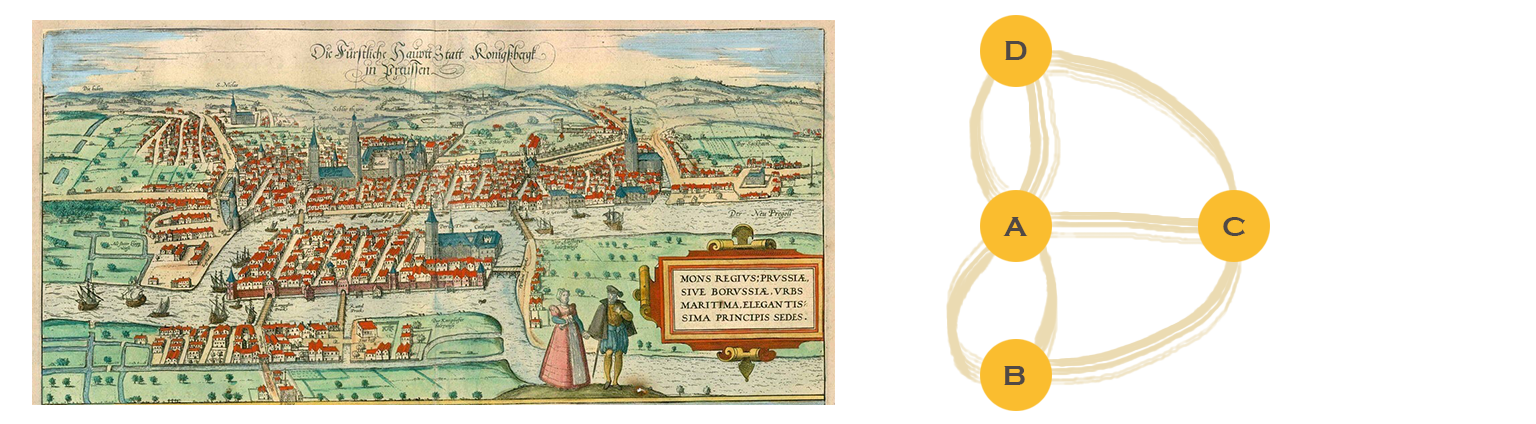
\includegraphics[width=14cm]{graphPnt.png}\hspace*{\fill}
        \end{center}
        Il est a noter qu'un tel graph est appelé un $2$-$graph$ en raison du nombre maximal d'arrete qui sorte d'un sommmet, mais dabord une defintion importants:
        \\
        \textbf{Graphe:}
          \emph{Un graphe simple $G$(S,A) est la donnees d'un ensemble fini $S$(pour sommet) ainsi que une partie $\mathfrak{P}_2(S)$ appeler A(pour arrets)}
        \subsection{Vocabulaire generale}
        \noindent\begin{minipage}{0.3\textwidth}% adapt widths of minipages to your needs
  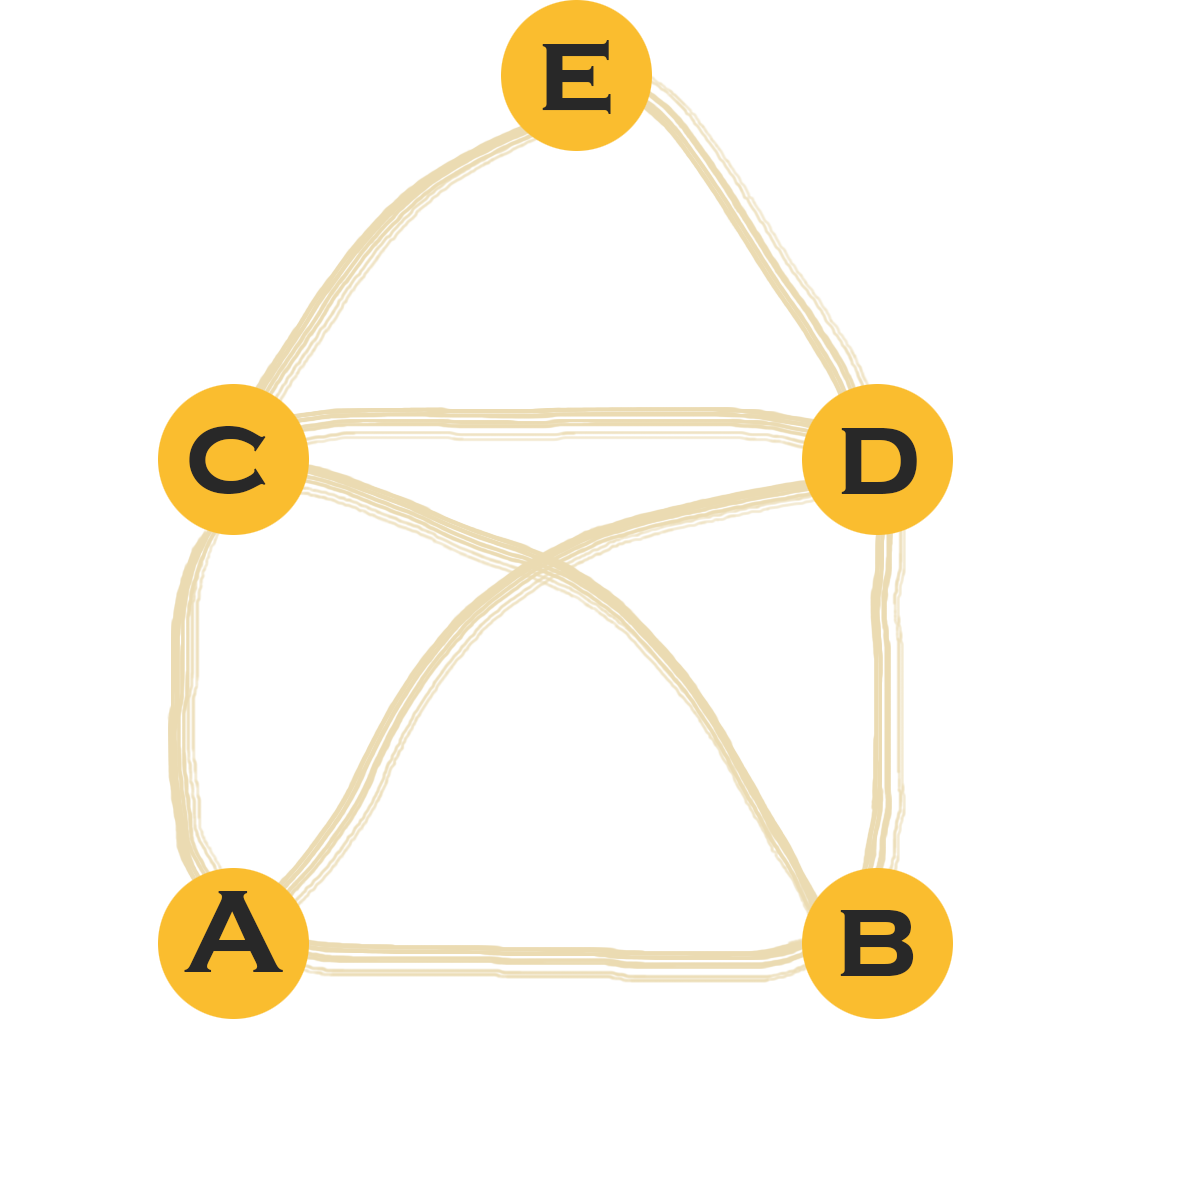
\includegraphics[width=\linewidth]{graphM.png}
  \end{minipage}%
  \hfill%
  \begin{minipage}{0.6\textwidth}\raggedleft
      $S$=\{a,b,c,d,e\}\\
      $A$=ec,ed,cd,ca,cb,db,da,ba\\
      graphe d'ordre 5\\
      a et b sont adjacent,\\ ac et cd sont incident
  \end{minipage}
    \textbf{Ordre:}
    \emph{Ordre d'un graphe et le nombre de ces sommets}
    \\
    \textbf{Adjacent:}
    \emph{deux sommet $a$ $b$ sont dit adjacent si il sont relier par une arrete commune autement dit:}\\
      $\{a, b\}\in A$\\
    \textbf{Incident:}
    \emph{On dit que deux arret $u$ et $v$ sont incident si il possede un sommet commun autrement dit:}\\
    $a \wedge b \neq \emptyset$\\
    \textbf{Chemin:}
    \emph{Un chemin de longueur n, est une suite de sommets telle que:}\\
    $\forall i, 0\leq i\leq n\Rightarrow x_i,x_{i+1},x_n\in A$
    \\\emph{note: si $x_0=x_n$ on parle plutot de cycle, de plus $x_n$ et $x_0$ sont appeler extremiter}\\
    \textbf{Chemin simple:}
    \emph{Un chemin de longueur n, est un chemin qui ne passe que une seule fois par chacune des ces arrete}\\
    \textbf{Chemin elementaire:}
    \emph{Un chemin de longueur n, est un chemin qui ne passe que une seule fois par chacun des ces sommets}\\
    \\De ce joyeux bordel de definition decoule deux autre concepte importants:
    \\
    \textbf{Chemin-Semi Eulerien:}
    \emph{Il s'agit d'un chemin qui passe par tout les \underline{arrete} une et une seule fois}\\
    \textbf{Chemin-Semi Hamiltonien:}
    \emph{Il s'agit d'un chemin qui passe par tout les \underline{sommets} une et une seule fois}\\
    On utulise uniquement le terme de semi car un vrai chemin ne l'est pas vraiment puisqu'il s'agit d'un cycle.
    \subsection{Parenthese NP-Complet}
      Un probleme peut etre selon la theorie de la complexite, facile ou dificile. Dans les fait cette distinction viens uniquement du faite de la complexite algorithmique. En effet un algo qui s'effecturas en un temps polynomiale seras considere comme facile a l'inverse un autre algorithme qui s'effecturas dans un temps superrieure seras appelé un algorithme dificile. \\On note qu'il existe des algo facile pour trouver si un chemin et Eulerien mais pas pour trouver si il est Hamiltonien de plus il s'agit d'un probleme NP-Complet.
    \subsection{Reduction et gadget}
    \begin{center}
     \hfill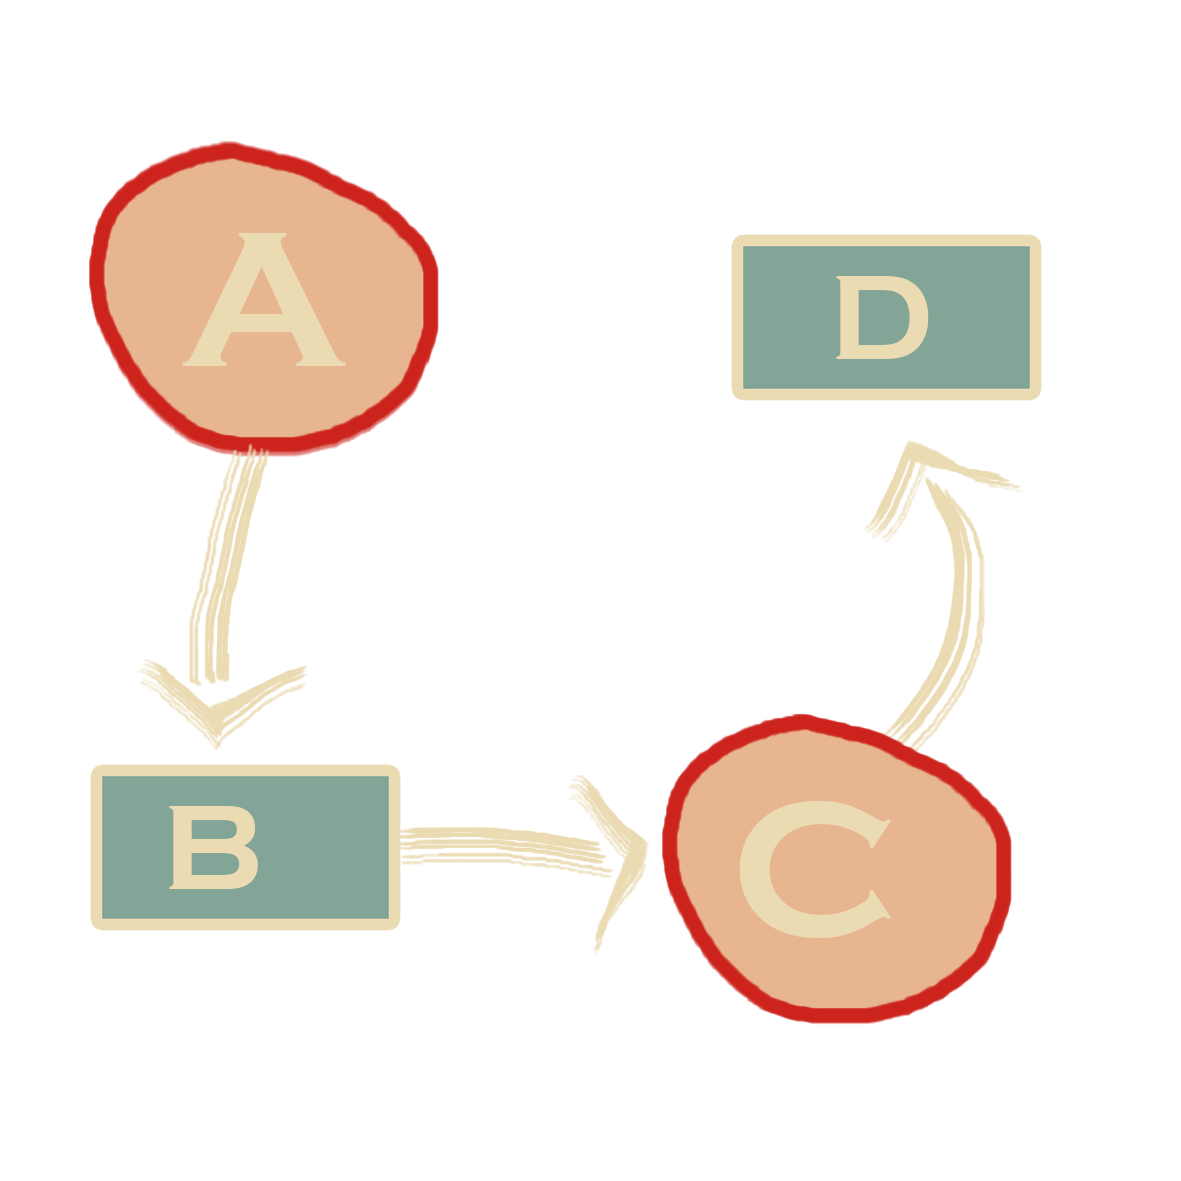
\includegraphics[width=5cm]{gadget.png}\hspace*{\fill}
    \end{center}
    Un gadget est une methode qui permet de resoudre un probleme de descidabilite, preno  l'exemple du probleme A qui n'est pas resoluble sans algo $difficile$(au sens de la theorie de la complexite)et prenont un un probleme C qui se resout $facilement$ avec un algo D ici un gadget ou reduction est un algo B qui transforme une instance du probleme A vers une instance du probleme B qui sera absolument equivalente.
    Par exemple savoir si un graph est Eulerien est une reduction de savoir si il est Hamiltonien.
    \subsection{Connexe}
    \textbf{Relation:}
    \emph{Dans un graph, deux sommets $s$ et $t$ sont dit relier entre eux si il existe un chemin d'extremiter $s$ et $t$}\\
    Une telle relation est symetrique, transitive, reflexive et est donc une relation \underline{equivalence}.
    Les classe d'equivalence de cette relation sont appeler des composante Connexe, la relation est decrite par le symbole $\rightsquigarrow$.
    \begin{center}
      exemple de composante connexe:\\
     \hfill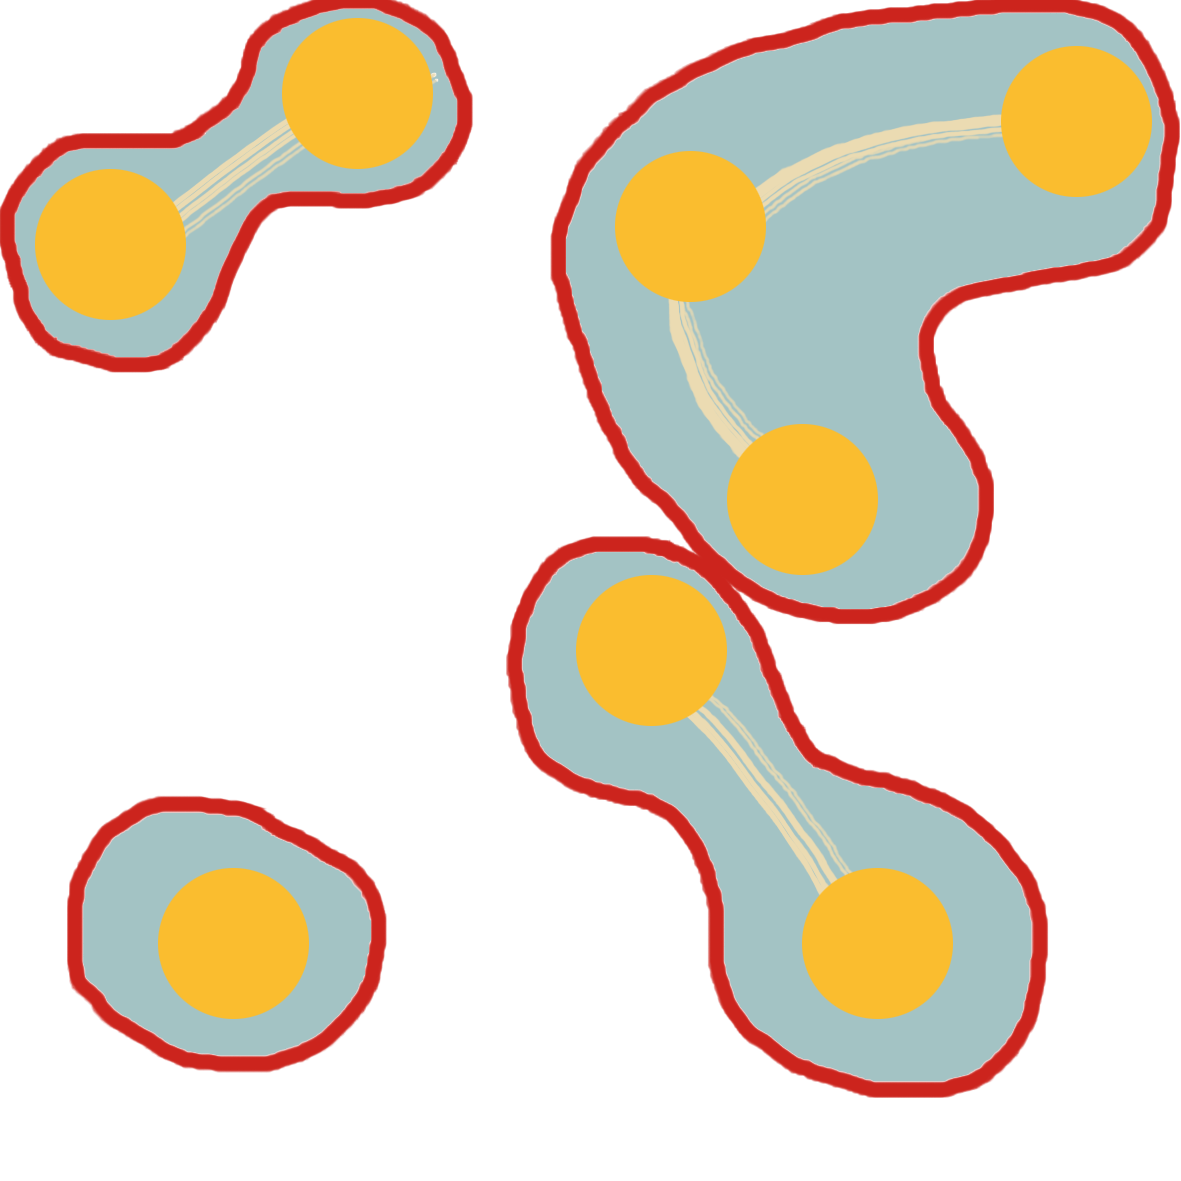
\includegraphics[width=5cm]{connex.png}\hspace*{\fill}
    \end{center}
    Un graph est dit connexe si pour chacun de ces sommets il existe un chemin vers n'importe qu'elle autre sommets.\\
    On note aue le degree d'un sommet est egale au nombre d'arret incidente
    \begin{center}
      \textbf{\color{LightOrangeHaf}Theoreme d'Euler:}
      \\Un graph G sans point isol\e \ et Eulerien ssi:\\
      \begin{tabular}{@{}l@{}}
        - il est connexe\\
       - tout les sommets sont pair\\
      \end{tabular}
    \end{center}
    \textbf{Demonstration du Theoreme d'Euler:}
    On se retouve avec un graph $\daleth$ (S,A)Eulerien\\
         \noindent\begin{minipage}{0.3\textwidth}% adapt widths of minipages to your needs
  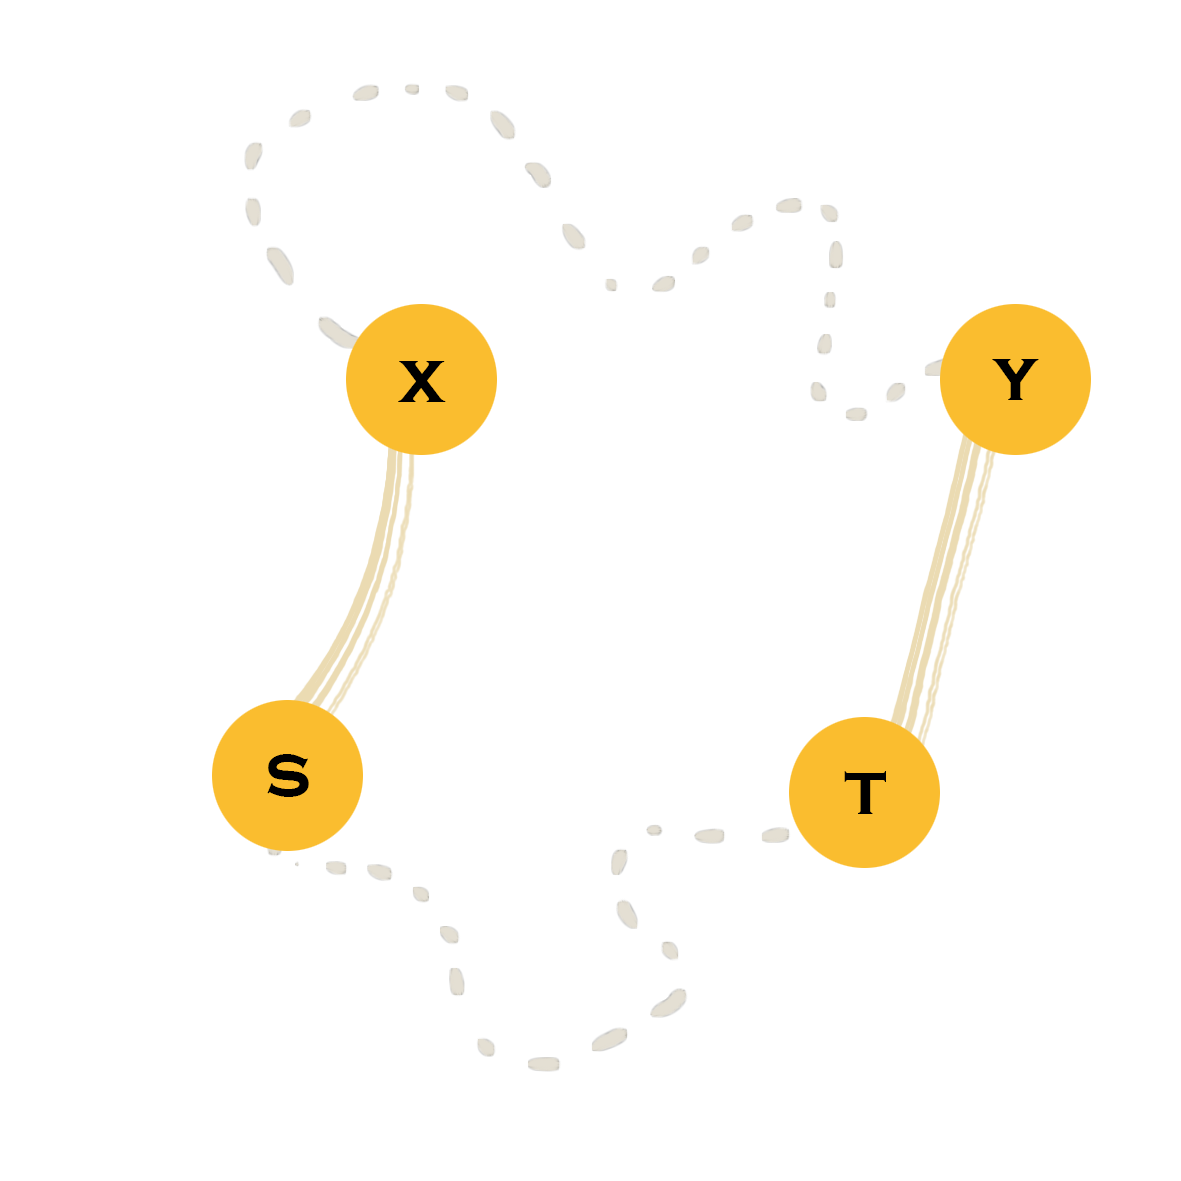
\includegraphics[width=\linewidth]{graphM3.png}
  \end{minipage}%
  \hfill%
  \begin{minipage}{0.6\textwidth}
      On condiere les 2 sommets s et t, ces deux sommet sont incident a des arrete et de plus il existe un chemin Eulerien qui passe par ces deux arrete et par s et de facto le graph $\daleth$ et connexe.
  \end{minipage}
    Ici le chemin et simple, de plus un cycle passe par tout les sommet donc le degree de chacun de ces sommets doit etre paire.
$\daleth$ (S,A) un graphe sans point isolem connexe dont les sommet sont paire.\\
  \noindent\begin{minipage}{0.6\textwidth}% adapt widths of minipages to your needs
    On part d'un sommet $x_0$ arbitraire et on construit un chemin  de proche en proche sans jamais passer deux fois par la meme arrete, on obtienderas evidament un cycle car les sommet sont pair.
  \end{minipage}%
  \hfill%
  \begin{minipage}{0.3\textwidth}
  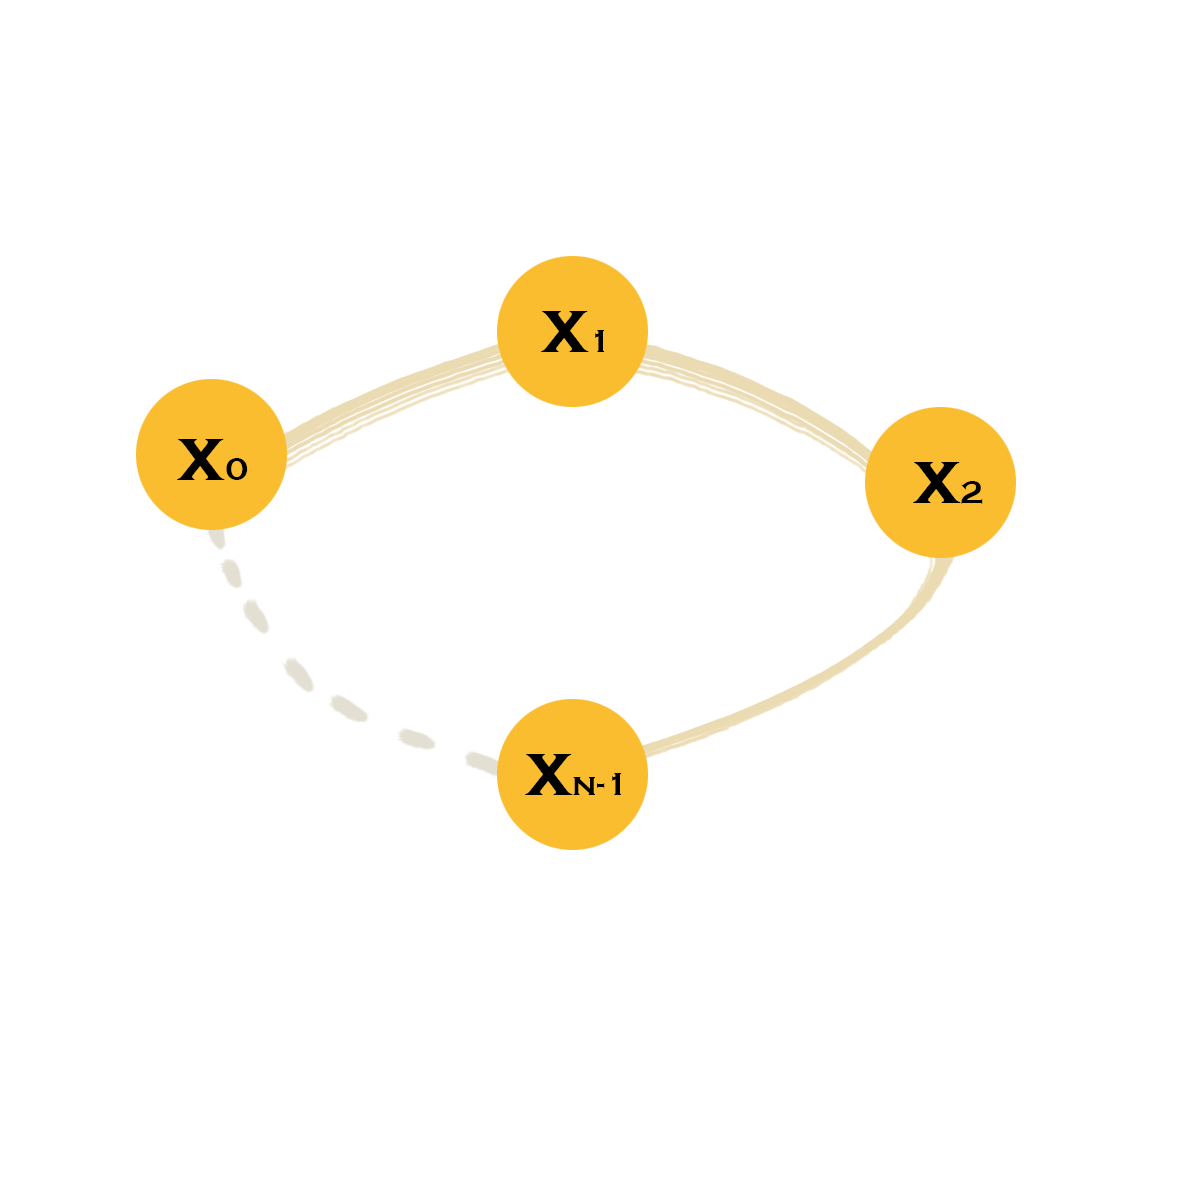
\includegraphics[width=\linewidth]{graphM4.png}
  \end{minipage}
  Observont le graph partielle de ce chemin:
  \begin{center}
  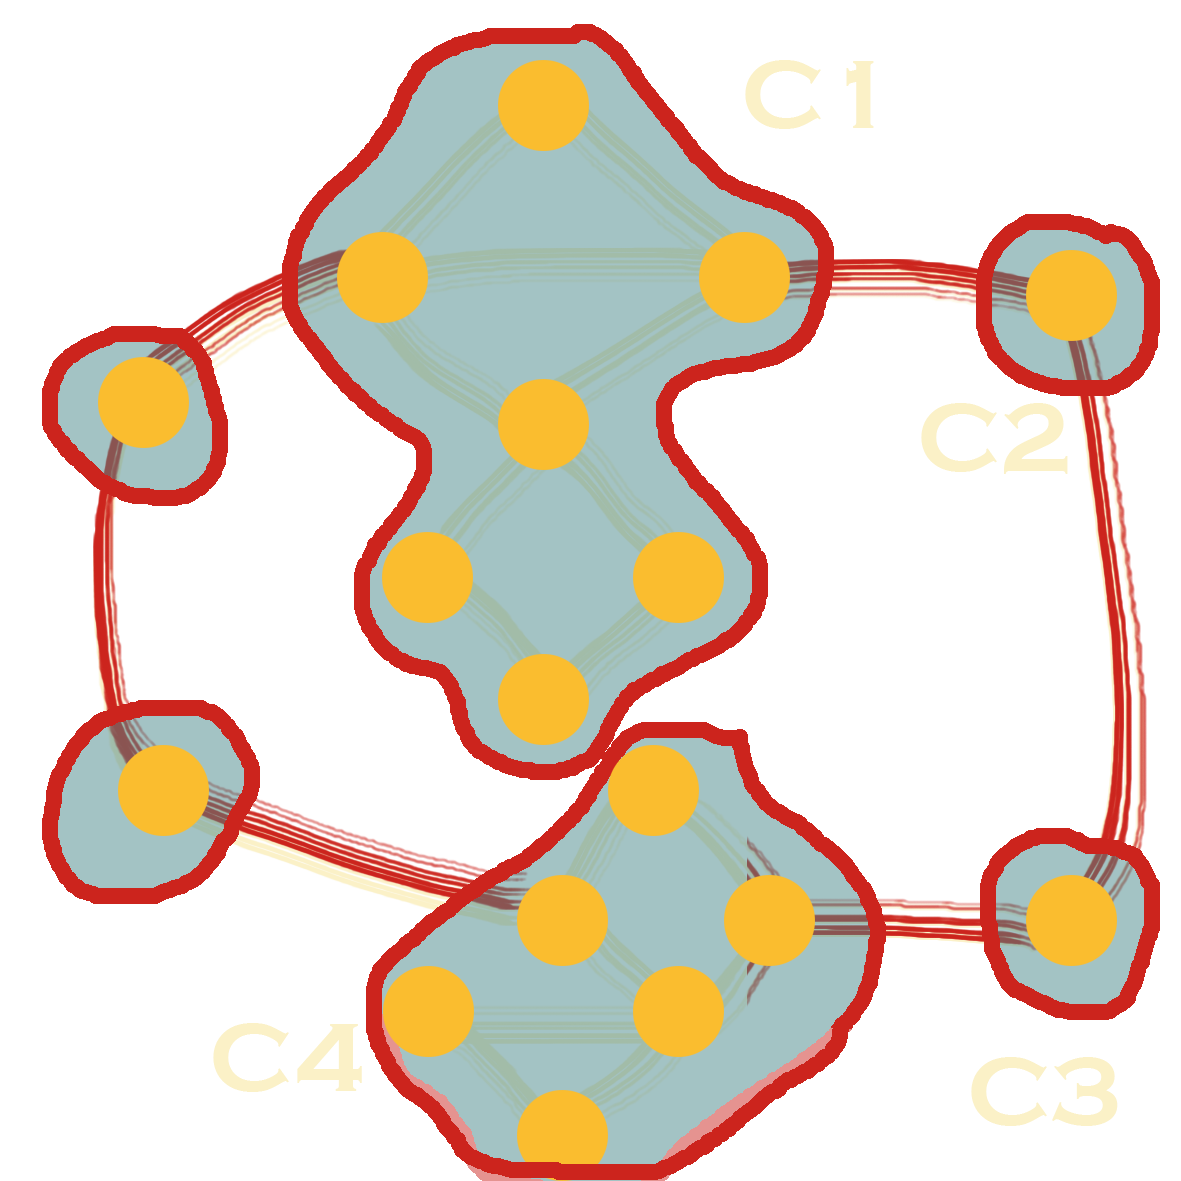
\includegraphics[width=6cm]{connex2.png}
  \begin{enumerate}
    \item $C_k$ est connexe
    \item tout les sommets de $C_k$ sont paire
    \item le nomebre d'arret de $C_k$ est strictment superrieure au graph initiale
  \end{enumerate}
  \end{center}
\end{document}